\documentclass[a4paper]{article}
\usepackage[top=13.5mm, bottom=13.5mm, left=10mm, right=10mm]{geometry}
\usepackage{tikz}

\begin{document}

\begin{center}
    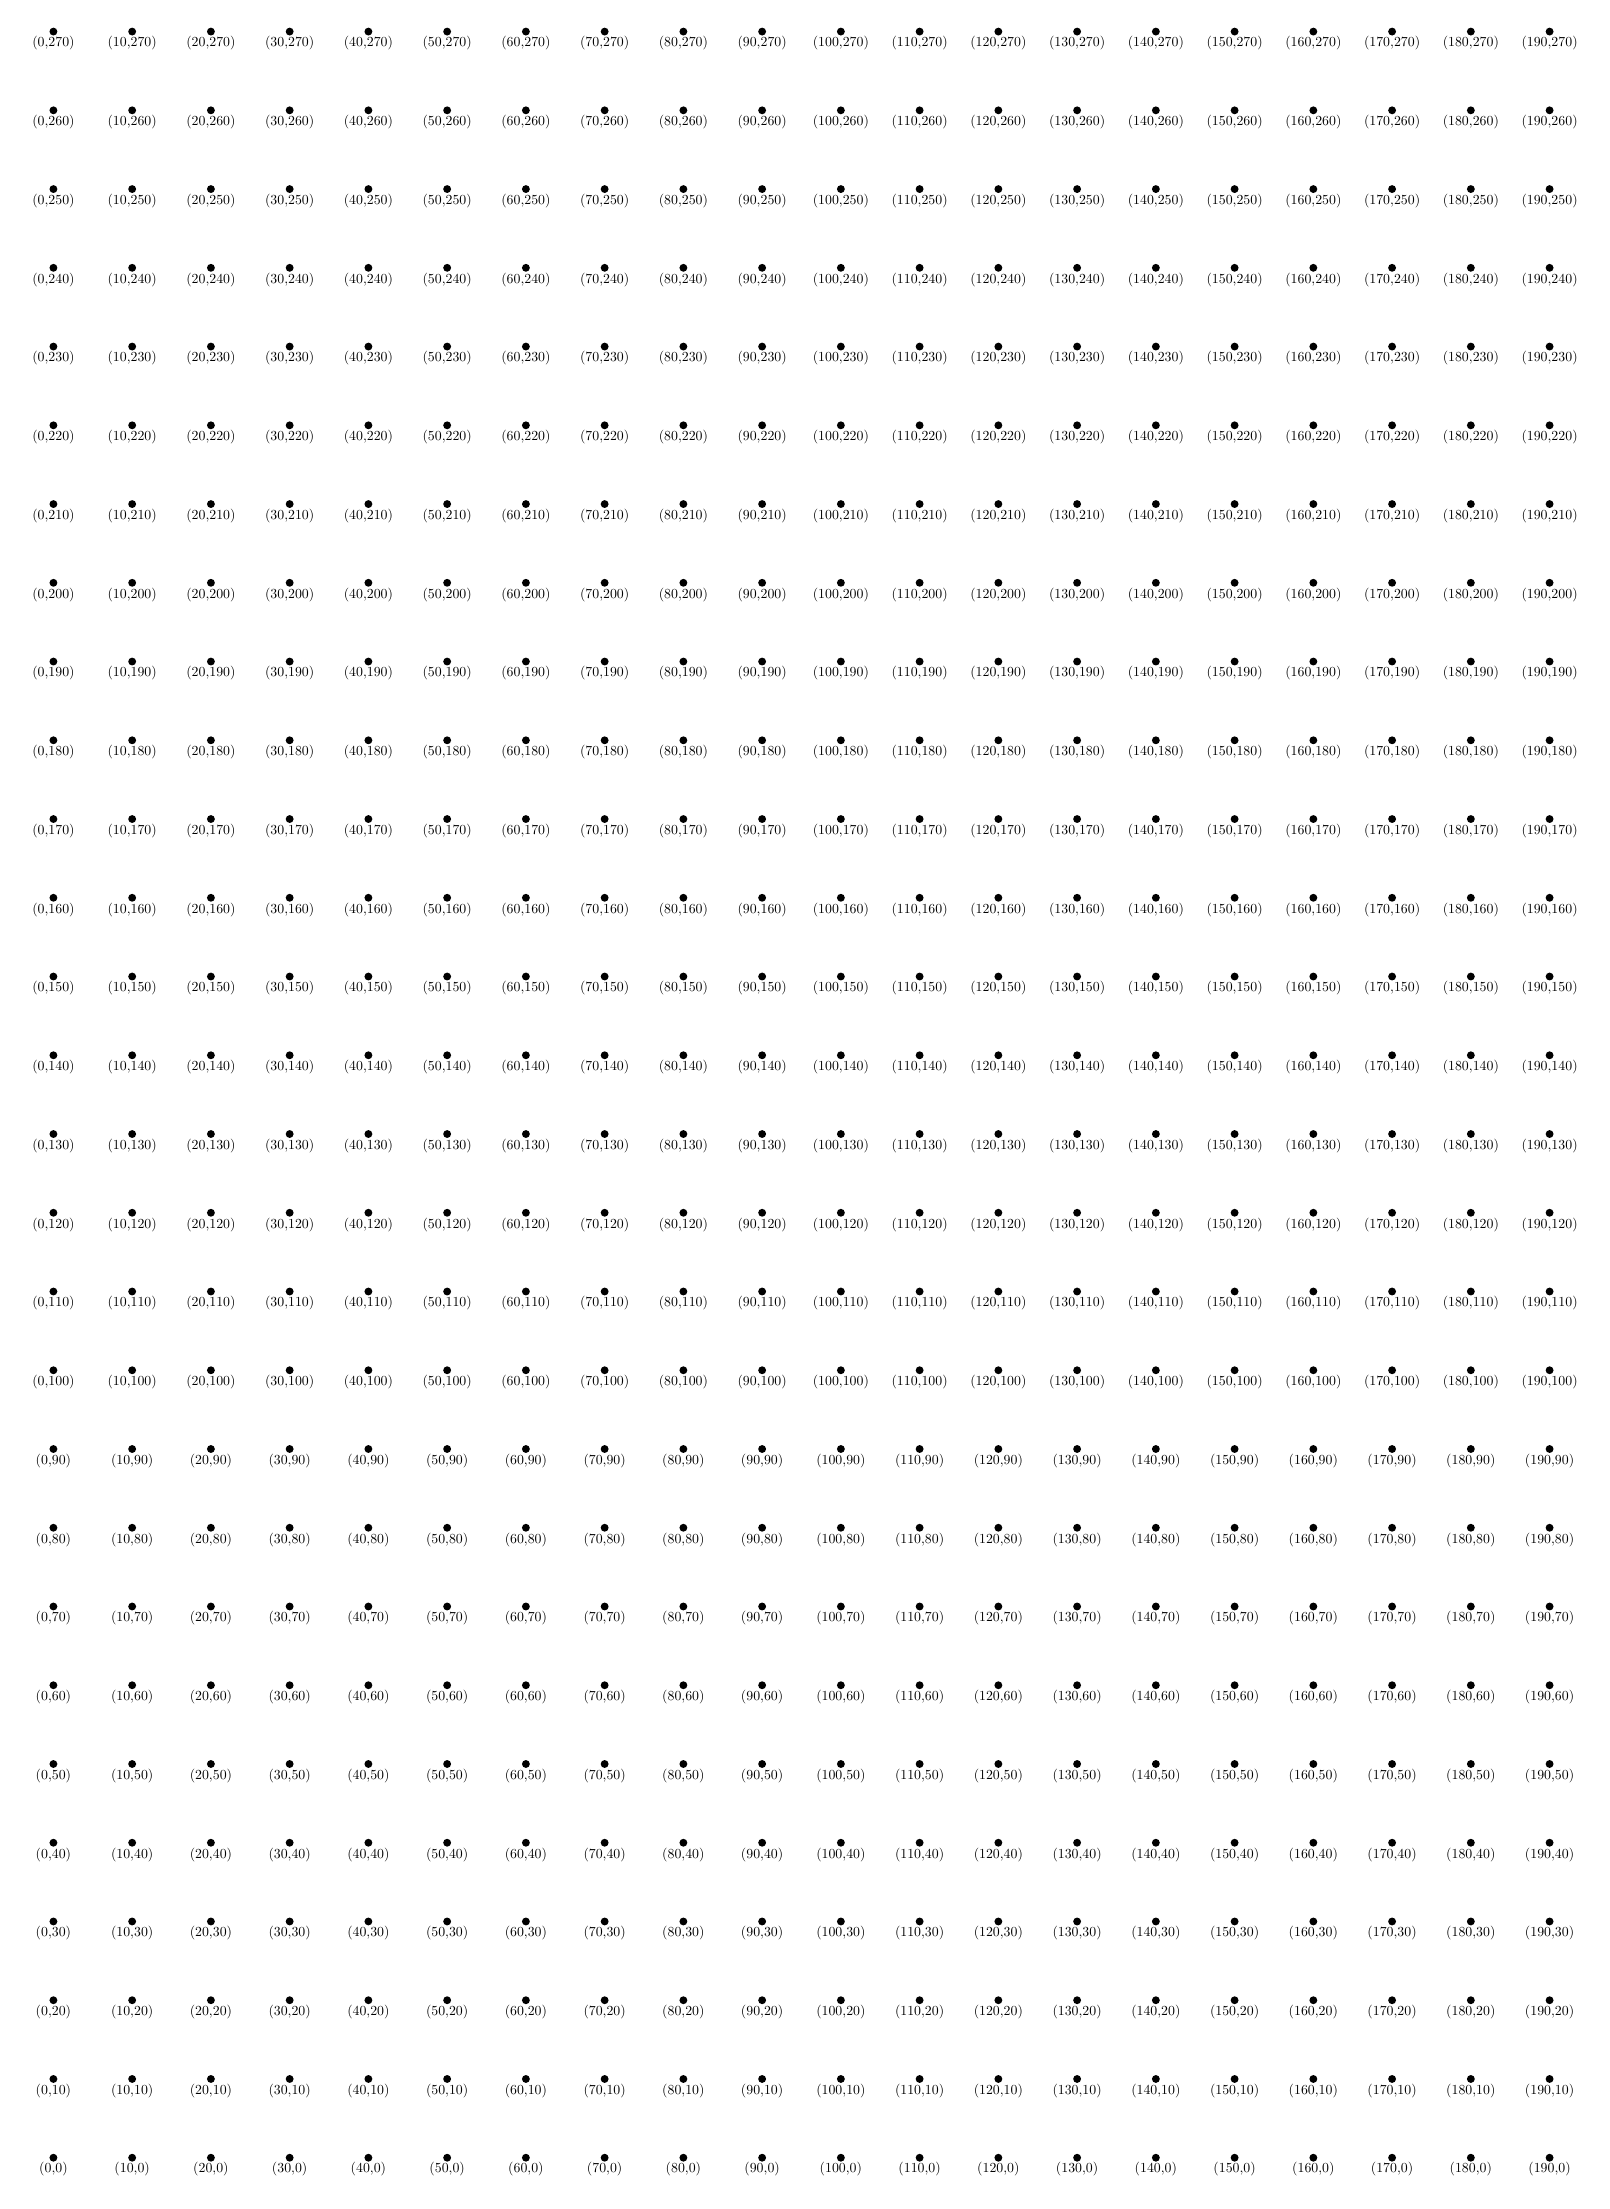
\begin{tikzpicture}[scale=0.1] % Scale to match mm units
        
        % Define A4 working area (after applying margins)
        \def\width{190}  % 210mm - left 10mm - right 10mm
        \def\height{270} % 297mm - top 13.5mm - bottom 13.5mm

        % Draw grid points every 10mm and label them
        \foreach \x in {0,10,...,190} {
            \foreach \y in {0,10,...,270} {
                \fill (\x,\y) circle (0.5); % Draw point
                \node[scale=0.5, anchor=north] at (\x,\y) {(\x,\y)}; % Label point
            }
        }

    \end{tikzpicture}
\end{center}

\end{document}
